% !Mode:: "TeX:UTF-8"
\chapter{移动社交网络中的关系识别分析}

\qquad 移动社交网络中的关系识别是当前主流研究课题之一。在一个特定的网络中,用户之间往往存在各种的社交关系,如家人、朋友、同事关系等等。明确社交网络中用户之间不同的关系类型,有利于其它领域的深入研究与发现。如在线或者移动广告营销中,如果知道用户家人、朋友的兴趣爱好以及其常购买的商品类型,那么就能更加准确的给该用户推荐相关的商品与广告,反之亦然,知道用户的喜好,也可以给其朋友、家人等推荐相应合适的商品。在协助公安侦破并抓捕犯罪嫌疑人时,如果能够掌握犯罪嫌疑人其家庭、朋友,则能更快协助相关部门侦破案件,有效的抓捕犯罪人员。由前面介绍可以得知,由于移动智能手机的普及率日益上升,使用移动手机(当然主要是智能手机)的人群覆盖率将近100\%, 具有一定的普适性。除此之外,移动运营商所提供了家庭套餐、集团套餐等营销套餐,如果研究者能够和移动运营商进行合作,则研究者能够利用从移动运营商中获得的关系数据,作为其训练数据。

从第二章可以得知,从机器学习的角度来看,关系识别问题为分类(Classification)。由前面的第二章节介绍可以知道,当前已经有相当多的学者在进行该方面的研究工作。然而,但绝大多数此类的研究工作都是将关系拆分为简单的“信任与不信任”,“朋友与非朋友”关系,并没有将这种抽象的概念放在一个具有明确关系语义的网络当中去(如具有家庭、同事、朋友的关系网)。还有部分研究对对关系分类赋予了特定的寓意,但这些研究主要有“辅导-被辅导”\upcite{wang2010mining}、“讲授-指导-助教”关系\upcite{taskar2003link},比较适用于有向关系,而并非特别适合本文所研究的家庭、同事和朋友关系集。另外一些研究则是基于特别的数据集,如恐怖分子网络数据集分布\upcite{zhao2006entity}, 和本文所要进行研究的通话网络数据结构和性质相差太大,并且这些性质的研究,大多仅从社交层面上对关系进行阐释,而不能从模型的角度充分挖掘社交与空间地理位置之间的联系,而本文所要做的工作则需要从这两个角度同时进行考虑。


移动社交网络提供了非常丰富的信息,可以用来挖掘人们在真实日常生活中的社交关系。在本章,本文首先对基于通话数据中移动社交网络的关系识别问题进行论述和定义,然后将本文所研究的数据进行详细介绍。最后,本文针对从用户通话角度、地理位置同现两个角度进行出发,研究不同交互特征下同事、家庭、朋友关系之间的显著差异,并对特征进行相应的分析。本文用通话数据展示本文的发现。由于篇幅的限制,本文不展示在短信息中的发现,但两者的特征发现比较相近。

\section{关系识别问题定义}
很显然,社交网络是一个图模型,因此不同的问题的基本构成都可以用图$G = (V, E, W)$来进行表示,其中网络图中的每个点$ v_i \in V$表示该网络中的用户,图中点与点的边$Edge(v_i, v_j) \in E$ 表示用户$i$与用户$j$之间存在某种联系(这种联系可以自己定义,如在本文的问题中即两人存在社交关系),而$W$则表示了这种点与点之间的关系强度(如在本文的问题中,则可以定量描述为两用户之间的通话频率与强度等)。

具体到本文的问题当中,本文让$G = (V, E, X, Y)$ 代表无向移动社交网络,这里的$V$ 是$|V| = N$数量的用户集合,而$E \subset V \times V$是表示用户之间社交联系边的集合,每一条边$e_i \in E$ 都有一个相应的社交关系$y_i \in Y$与之对应,这里的$Y \in $\{家庭关系, 同事关系,朋友关系\}。需要注意的是,这里的朋友关系定义为联系较为频繁的用户。$\textbf{X}$是特征矩阵,$\bm{x_i}$代表了$|\bm{x_i}|$维特征向量,为每条边$e_i$的特征。因此在解决最终问题,推断移动社交网络前,本文需要选取合适的特征,即$\bm{x_i}$的值。



\section{数据介绍}
在本论文中所使用的数据集是从2010年10月1日到2010年10月25日采集的中国河南省某县级市的移动手机通话短信数据,包含了30万用户超过六千万(67,630,000)条的通话记录,三千万(31,560,000)条的短信记录,四百万(4,420,000)条的手机开关机纪录,一千二百万条的基站切换纪录。该县级市总共有354座基站,而且每一座基站都有相应的经度和纬度。具体的数据内容格式在表3.1。开机和关机、通话基站的切换数据格式如表3.2.




除此之外,本文的数据当中有由移动运营商提供的家庭(Family Clique)和同事集团(Colleague Clique)的具体关系。为了更加精确、更加合理的预测用户之间的关系类别,本文移除了那些家庭集团和工作集团大小为1的孤立点,因为这些点不会对本文所分析的问题构成任何贡献(本文研究的问题本身就是边的关系)。除去这些无用的用户之后,本文可以发现大多数的集团由两个或者三个构成,这类型的集团占了所有家庭和同事集团总数的83\%。并且本文从数据分布上可以发现,同时集团的大小大多小于10人。


\begin{table}
    \centering
    \caption{短信/通话数据格式}
    \label{call-record}
    \begin{tabular}{c|c|c|c|c}
        \hline
        主拨号码 & 接听号码 & 通话时长 & 主拨用户所在基站 & 接听用户所在基站 \\ \hline
        1597128XXXX & 1565295XXXX & 2010-10-20 18:12:34 & 60234 & 60183 \\ \hline
    \end{tabular}
\end{table}


\begin{table}
    \centering
    \caption{事件纪录格式}
    \label{event-record}
    \begin{tabular}{c|c|c|c|c}
    \hline
    事件发生时间 & 用户手机号码 & 时间类型 & 起始基站 & 终止基站 \\ \hline
    2011-10-20 10:10:13   & 135XXXXXXX & 1 & 60284 & 74856  \\ \hline
    \end{tabular}
\end{table}


\begin{figure}[ht]
    \centering
    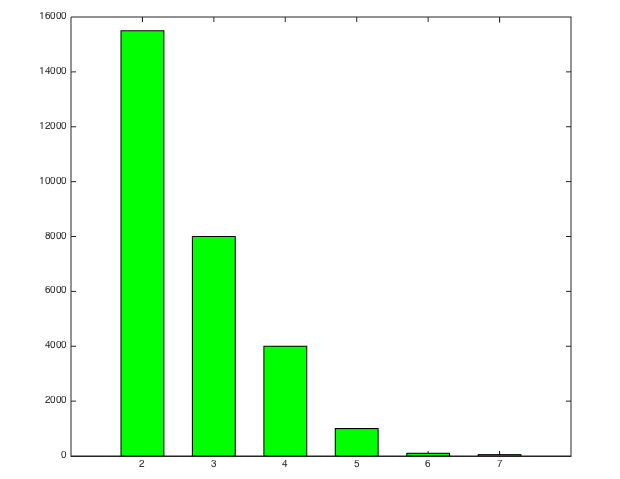
\includegraphics[scale=1,width=0.7\textwidth]{figure/FamilyClique.png}
    \caption{家庭集团大小分布}
    \label{fig-familyclique}
\end{figure}

\begin{figure}[ht]
    \centering
    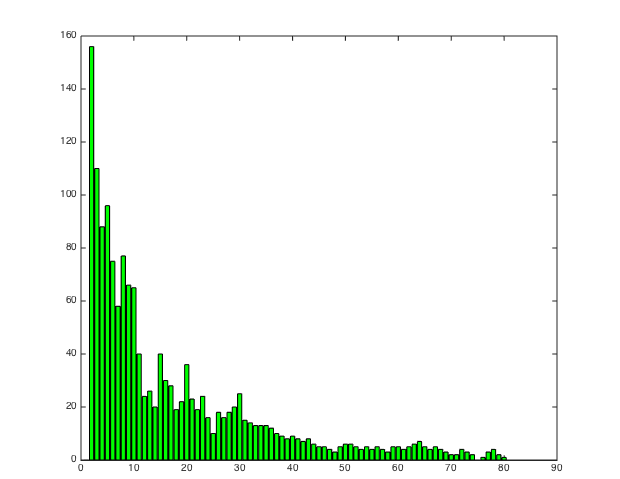
\includegraphics[scale=1,width=0.7\textwidth]{figure/ColleagueClique.png}
    \caption{同事集团大小分布}
    \label{fig-colleagueclique}
\end{figure}



\section{社交关系识别中的特征分析}

本节主要从移动社交网络中的用户交互、时空交互、社交与时机地理空间交互等角度来分析影响社交关系识别的关键特征,充分利用移动社交网络的社交、空间结合等特性。本小节先从通话社交的角度进行分析,主要分析基本的通话特征对关系识别的影响,以及引入通话熵的概念,然后分析不同关系用户之间时间和通话强度的稳定性与差异性。然后从时空交互的角度来分析,分析了用户时空同现性。随后,分析用户出现地理位置的寓意分析,了解用户同现所在实际位置的具体含义。最后,从经典的社交结构论扩充到地理空间的范围内,提出新的结构洞理论。

\subsection{基本社交通话特征行为分析}

从以前的研究中,本文可以知道,通过用户的通话记录,用户之间的关系(朋友、非朋友)能够很好的被识别出来\upcite{min2013mining}。但在那篇文章所用到的数据集都非常的小,并不能代表用户交互之间公共的特点,并不能直接认为围绕通话记录所得到的通话特征行为在本文的数据集上也有同样的效果。因此,本文在本文文章的数据集中重新考虑了用户之间的通话记录对关系识别的影响。

在图3.3中,本文分析了不同的社交关系在一天之内,不同小时段的通话概率分布情况。这里本文定义忙时为每天的10AM到12AM,6PM到9PM期间。可以看到,无论哪儿种关系,在通话整体分布上呈现双峰分布,而曲线的最高点即为每天的忙时期间。在图中本文不难发现到,那些具有家庭关系的用户会比具有同事关系的用户拥有更高的交流通话频率。除此之外,本文也可以观察到,家人之间往往会选择在忙时进行通话。而具有同事关系的用户,往往选择的是在工作时间段(每天的9点到12点,以及下午14点到18点)内进行通话,而到了下班时间,本文会选择与具有家庭关系的用户进行通话,很有可能要通知家人是否要回去吃晚餐,大概几点会到家等话题。另外,朋友关系并不具有很明显的时间段分布,这反映了朋友关系往往是有事了才会选择通话,而并不具有每日特定时段的规律性,反映了朋友通话的随机性。从中本文可以知道,不同社交关系在不同时段之间的通话关系在一定程度上,反映了本文日常的行为,如从上述分析中本文可以知道人们往往会在下班之后选择和家人进行通话。这也充分反映了通话行为在识别不同社交关系的有效性。



\begin{figure}[ht]
    \centering
    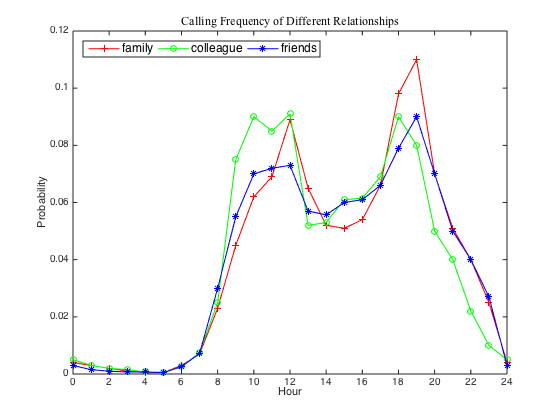
\includegraphics[scale=1,width=0.8\textwidth]{figure/callFrequencyDistribution.png}
    \caption{社交关系与不同小时段通话频率之间的联系}
    \label{fig-callFrequency}
\end{figure}

从日常生活经验中,本文可以知道,人们在周末和工作日的通话行为往往是不一样的,为此,有必要分析不同社交关系在工作日和周末的通话行为。如图3.4,图(a)为在工作日的不同社交关系通话频率分布差异,图(b)为在周末不同社交关系的通话频率分布差异。除了在上述图3.3的分析中所发现的特性,本文分析工作日和周末通话频率的共性和差异可以知道,不管是星期天还是周一到周五,具有家庭关系用户们之间的呼叫频率都远远的超过具有同事或朋友关系的用户,这也充分体现了人们往往与自己的家人联系频繁。在周末,具有家庭、同事两种关系的用户,相对于工作日,两类关系的通话频率均有下降。这并不难发现,在周末家人大多数时间都是呆在一块,并不需要通过电话来进行联系。而同事之间在休息日若无工作,则很少通过电话来进行沟通。而朋友关系,正如在图3.3中所发现的,在周末和工作日的分布较为平稳,没有很大的区分,这也反映了朋友关系之间的稳定性。


\begin{figure}[!ht]
    \centering
    \subfigure[工作日通话频率分布]{
        \label{fig-call-weekday}
        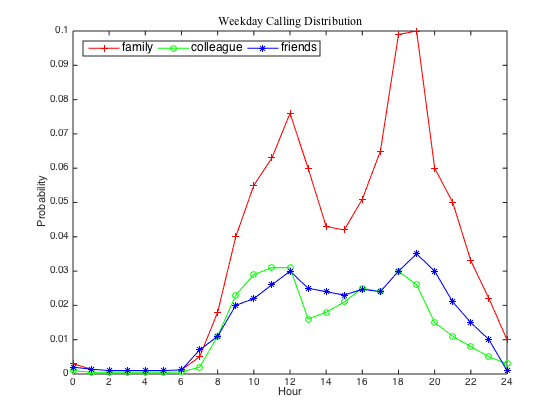
\includegraphics[width=.8\textwidth]{figure/callFrequencyWeekDayDistribution.png}
    }
    \hspace{7em} % 水平间隔
    \subfigure[周末通话频率分布]{
        \label{fig-call-weekends}
        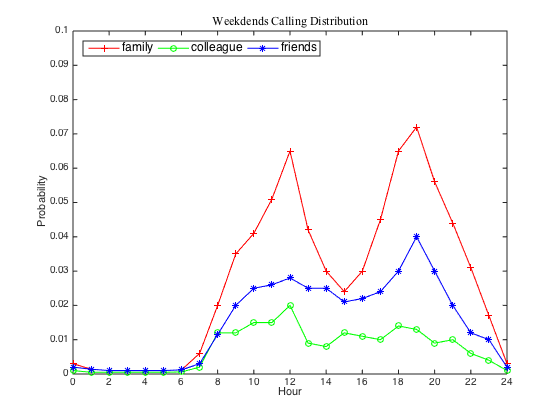
\includegraphics[width=.8\textwidth]{figure/callFrequencyWeekendsDistribution.png}
    }
    \caption{社交关系与不同小时段通话频率之间在工作日与周末的区别与联系}
    \label{fig-sub}
\end{figure}

\subsection{通话熵分布分析}

本文知道,本文会在不同的时间段内与不同的人通话联系。通常人们会在他们工作的时间与他们的同事通过手机联系。虽然说家人们主要集中在忙时通话,如下班之后。但是大多数的人们如果需要和他们的家人联系则不会等到某个特定的时间段内再联系,而是会直接打电话联系。为了定量描述这一特性,本文提出了通话熵的概念,可以用来描述用户之间通话的稳定性。熵的概念来源于信息领域,常常用来描述变量的随机性。由熵的概念而联想到的,本文定义了,通话熵的概念,用来描述通话在时间分布上的随机性。

\begin{definition}
    \label{call-entrpy-concept}
    \textbf{通话熵}计算公式,
    \begin{equation}
        CallEntropy = - \sum_{i=1}^{T}p(x_i)\cdot\log p(x_i)
    \end{equation}
\end{definition}


其中,$p(x_i)$ 为了用户第$i$小时段内通话的概率,$T$的值设置为24,代表一天有24小时。如果计算结果Call Entropy的值小,那么说明移动通话用户的通话时间分布相对集中,这也意味着他的的通话分布相对比较稳定一些。反之,如果用户的通话熵越大,那么用户通话的时间越分散,即反映了该用户群体的通话时间越不确定。


\begin{figure}[!ht]
    \centering
    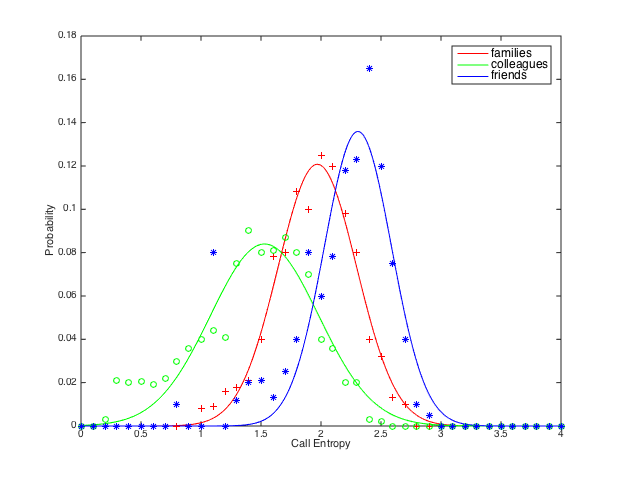
\includegraphics[scale=1,width=0.9\textwidth]{figure/CallEntropyDistribution.png}
    \caption{社交关系与通话熵之间的联系}
    \label{fig-call-entropy}
\end{figure}


在此概念的基础上,图3.5统计了不同社交关系用户的平均通话熵分布。通话熵分布都遵循高斯分布。但是,具有朋友的社交关系的通话熵值是最大的,而具有家庭关系的用户的通话熵值小一些,而同事关系的通话熵值是最小的。这一现象揭示了同事之间往往会选择在特定的时间段(从前面的分析中本文可以知道主要在工作时间段内)进行通话,而家人和朋友则更多会随意一些。这也充分证明了朋友关系是作为一种非常重要的社交关系,因为人们在想起了事情或者想朋友了就会随时给他们打电话。这一区分度非常符合本文在实际生活中的通话习惯,以及处理不同社交关系的基本策略等等。

\subsection{空间位置同现性分析}

与传统的社交网络相比,移动社交网络不仅仅能够揭示用户之间基本通话行为所具有的特性,更能够从他们的地理位置分布等角度来挖掘新的特性。在本文的数据中,正如前面所介绍的,每一次用户的通话和短信,开关手机时,用户所在最近的基站都被记录了下来。由此,本文就能够得到用户每次呼叫的地理位置信息。基于这一其它社交网络并不具备的优势,本文进行分析不同社交关系与他们所具有的空间特征之间的联系时,具有得天独厚的条件。

如图\ref{fig-position-stamp},本文统计了用户的位置间隔分布,可以看出,绝大多数的用户记录间隔都在一个小时之内,这也表明本文的数据集记录比较频繁,可以用来研究用户的出行行为。

\begin{figure}[ht]
    \centering
    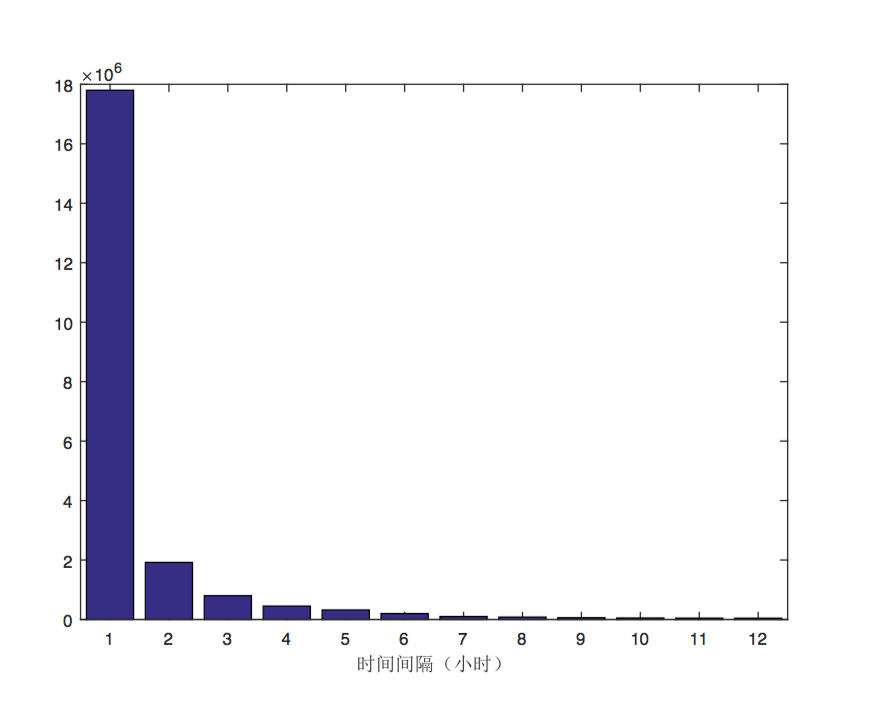
\includegraphics[scale=1, width=0.7\textwidth]{figure/timestamp.PNG}
    \caption{数据集中的用户位置间隔}
    \label{fig-position-stamp}
\end{figure}


接下来本文对用户的位置同现条件进行定义。这里的位置同现不同于字面上理解的两人在同一时刻出现在了同一地点,因这一类的数据在整个数据集上的分布较少,同时本文也无法确定同一地点的具体含义,因此本文需要重新定义同一时刻,即时间相邻的时间段,以及统一地点,即空间相邻的地理范围。在以前的研究中,以小时为时间粒度进行聚合,算作时间相邻,算是一种比较有效的手段\upcite{wang2011human}。另外考虑空间相邻的定义,为了得到用户的地理位置,本文往往是考虑用户所使用的基站的位置,因此只要两个不同的用户使用同一个基站,就可以认为他们在空间上具有位置同现的特性。但是,在真实世界中,因为有的地方基站分布较为密集,即是两个人处于确切的同一位置,他们也有可能暴露给两个不同的基站,因此很有必要合并一些距离非常近的基站。因基站合并算法在当前研究中较为成熟\upcite{aurenhammer1991voronoi},本文采用当前已经由的基站合成算法,不再进行研究,用为$Voronio$ 图的基站临近合并算法\upcite{aurenhammer1991voronoi}。在进行这些工作之后,如果两个用户在一小时的时间间隔内处于同一基站下(合并之后的基站),那么本文可以认为,这两个用户时空位置同现。



\begin{figure}[!ht]
    \centering
    \subfigure[工作日不同社交关系同现特征分布]{
        \label{fig-spatialhomo-weekday}
        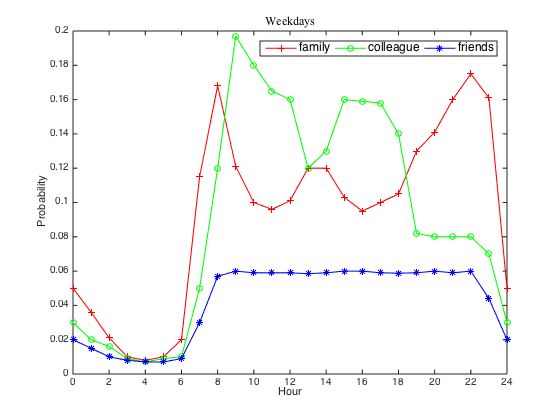
\includegraphics[width=.8\textwidth]{figure/spatialHomoWeekday.png}
    }
    \hspace{7em} % 水平间隔
    \subfigure[周末不同社交关系同现特征分布]{
        \label{fig-spatialhomo-weekends}
        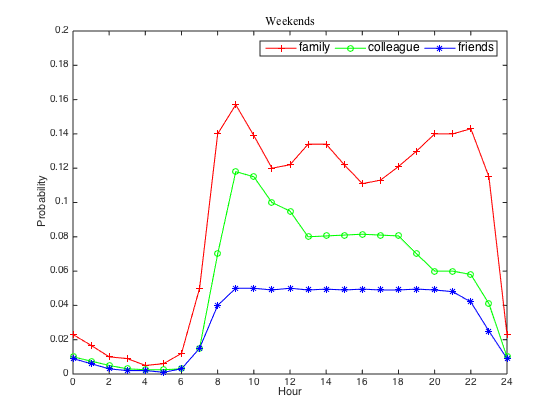
\includegraphics[width=.8\textwidth]{figure/spatialHomoWeekends.png}
    }
    \caption{社交关系与位置同现特征在工作日与周末的区别与联系}
    \label{fig-spatialhomo}
\end{figure}

图\ref{fig-spatialhomo}则显示了不同社交关系的用户在一天内同现的可能性分布,图\ref{fig-spatialhomo-weekday}为在工作日的同现特征分布,图\ref{fig-spatialhomo-weekends}为在周末的同现特征分布。图中横坐标为一天中的24小时,纵坐标为同现概率,这里本文定义同现概率。



\begin{definition}
    \label{spatial-homo-concept}
    \textbf{同现概率}定义,
    \begin{equation}
        C^{h}(x,y) = \sum_{l \in L}p_{x}^{h}(l) \times p_{y}^{h}(l)
    \end{equation}
\end{definition}


其中$L$ 为基站总集合,$p_{x}^{h}(l)$ 代表了用户$\bm{x}$在时刻$h$内出现在地理位置$l$的概率与可能性。

从图中的曲线本文可以观察到,无论在工作日还是在周末,三种社交关系在早上0点到4点的概率较低,其他时间以及在Weekdays和Weekends都呈现一定程度上不同的特征。在Weekdays的时候,同事在一起比其它关系的可能性要高。但是在工作日的中午,具有家庭关系的用户同现的概率反而增加了,而同事之间同现的概率出现了一个小的低谷状态。分析其中缘由,本文不难发现这个现象只有在中国小城市里面的传统家庭才会出现的。和许多国内外大城市不同的是,在中国中小城市里的人们往往会选择中午回家吃饭,并且进行短暂的休息。本文的数据集以及曲线很好地验证了这一现象。而在周末,家庭关系的用户同现的可能性最高,而朋友关系的用户同现可能性最低。这揭示了人们往往会在周末陪伴家人,呆在一起,而同事之间周末有时候会选择聚会等等活动。这些在曲线上所挖掘出来的信息,在现实生活中都得以体现,证明本文所提出来的同现特征,在本文的数据集上对关系识别有着很好的的效果,在一定程度上能对关系识别进行有效的区分。因此,本文可以进一步在同现特征的基础上进行扩展,挖掘出更多基于此思路的同现特征。



\begin{figure}[!ht]
    \centering
    \subfigure[工作日不同社交关系在出现最频繁的基站同现特征分布]{
        \label{fig-spatialhomoMost-weekday}
        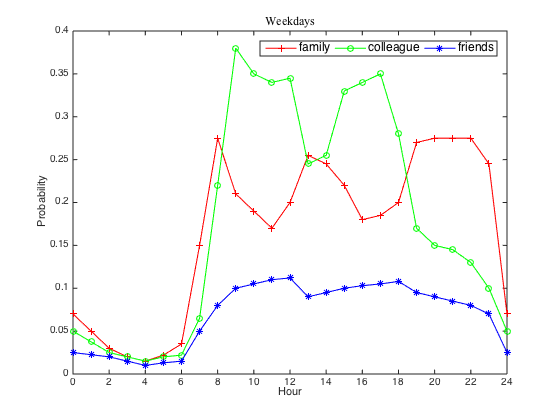
\includegraphics[width=.8\textwidth]{figure/spatialHomoMostWeekdays.png}
    }
    \hspace{7em} % 水平间隔
    \subfigure[周末不同社交关系在出现最频繁的基站同现特征分布]{
        \label{fig-spatialhomoMost-weekends}
        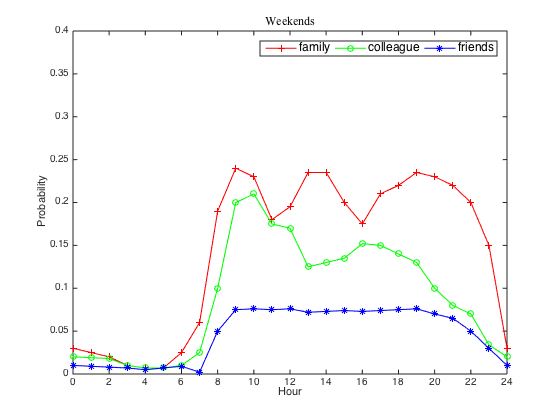
\includegraphics[width=.8\textwidth]{figure/spatialHomoMostWeekends.png}
    }
    \caption{社交关系与在最频繁出现的位置同现特征在工作日与周末的区别与联系}
    \label{fig-spatialhomoMost}
\end{figure}


从前面的分析中本文知道,从用户的总体轨迹的同现特征能够发现一定的规律。接着,本文分析用户出现最频繁的基站所附近同现特征的规律。从实际生活中本文可以得知,如果一个用户有工作,那么他在白天出现最频繁的基站很有可能就是他工作的地点附近。而晚上出现最频繁的基站则很有可能就是他家里面,所以单独选出着用户出现最频繁的基站有很大研究意义。由于时间和篇幅的限制,这里仅仅对用户出现最频繁的基站进行分析,而并非分为用户在白天和夜晚出现最频繁的基站进行研究。这里对一些概念来进行定义,$l_x^h$为用户$x$在$h$时出现可能性最高的基站,基站同现的概率

\begin{definition}
    \label{spatial-homoMost-concept}
    \textbf{最频繁基站同现概率}定义,
    \begin{equation}
        P^{h}(x,y) = (l_x^h == l_y^h)? 1:0 
    \end{equation}
\end{definition}

如图\ref{fig-spatialhomoMost}即为不同社交关系在最频繁出现的基站的概率统计。可以观察到,在工作日,具有同事关系的用户在白天同现率较高,而具有家庭关系的用户在晚上在最频繁基站具有较高的同现率。这也验证了本文之前的猜想,本文在白天一般出现最频繁的位置就是本文的工作地点,而晚上出现最频繁的地点则为家所在的地点。而在周末,具有家庭关系的用户同现率也比较高,这也验证了前面的结论:人们周末更愿意花时间陪伴家人,而且更愿意在家里面和家人相聚。



\subsection{空间地理语意分析}

前面的分析本文主要从同现的角度来分析用户的特征行为,得到了一些有用的结论。接下来的分析,本文希望能够深层次的探讨不同关系用户出行的规律与含义。本文现在知道,用户拨打和接收电话的记录记录了每个用户所在的基站的信息,而每个基站都有相应的经纬度信息。直观上看这些经纬度信息除了统计实际物理世界的地理位置分布之外,并无其他作用。但是由于移动互联网的发展,有了基于位置的服务。从这些基于位置的服务(Location Based Service)中,本文可以得到一些有实际意义的信息。

结合本文特有的国情,本文使用地理位置服务提供商百度地图(中国最大的LBS提供商)获取基站范围内的$POI$(Point of Interest,地理热点)信息,对于输入的经纬度信息,百度地图API返回一个响应的数据如图\ref{fig-baidu-poi}所示。



%\begin{figure}[ht]
%    \centering
%    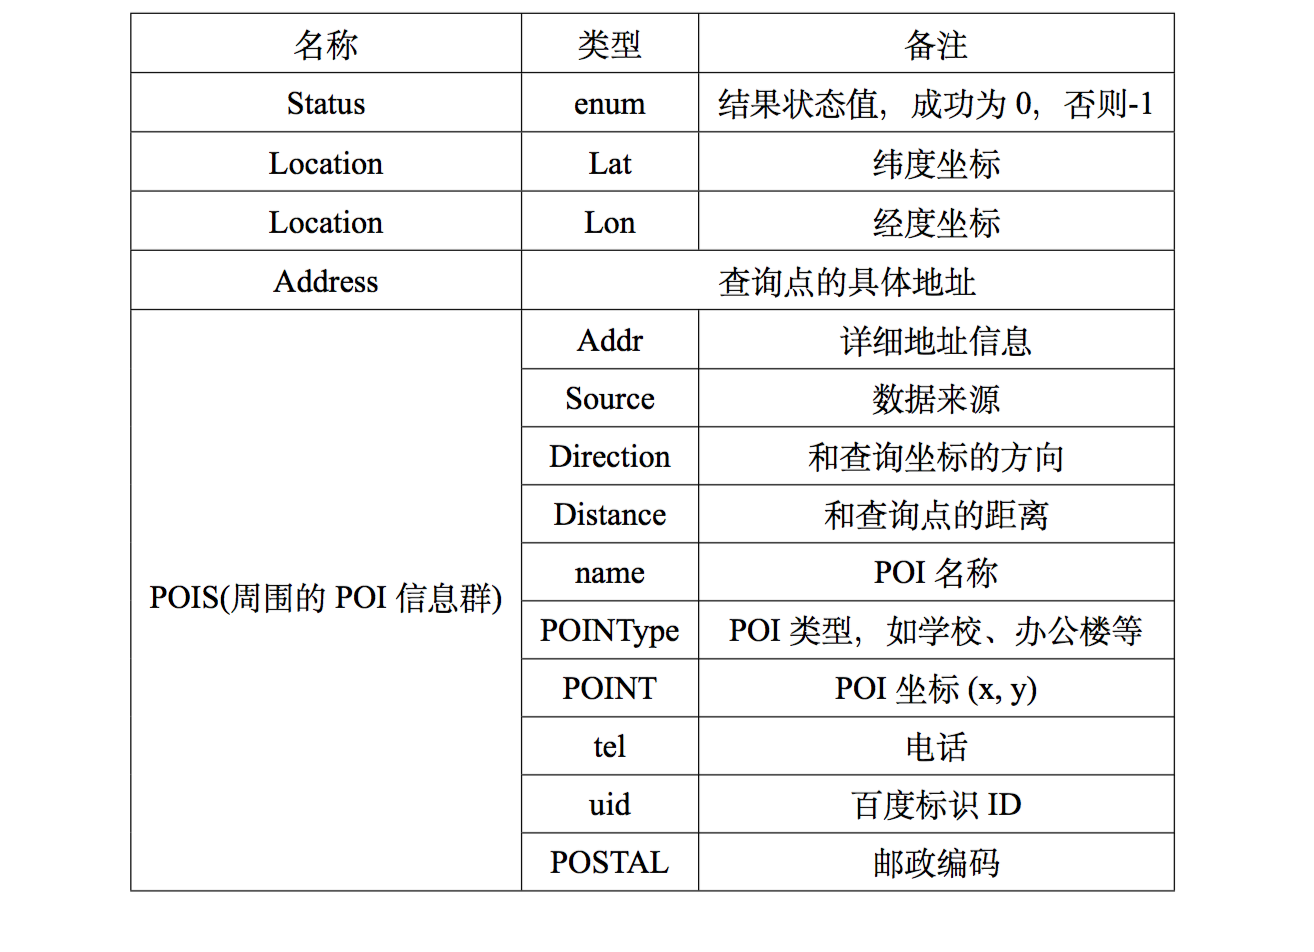
\includegraphics[scale=1, width=\textwidth]{figure/baiduAPI.PNG}
%    \caption{百度地图API返回POI信息}
%    \label{fig-baidu-poi}
%\end{figure}



\begin{table}[ht]
    \centering
    \caption{百度地图API返回POI信息}
    \label{tab-poi-info}
    \begin{tabular}{c|c|c}
        \hline
        名称 & 类型   & 备注                    \\ \hline
        Status & enum  & 状态值,正常0,否则-1 \\ \hline
        Location & Latitude & 纬度坐标               \\ \hline
        Location & Longitude & 经度坐标               \\ \hline
        Address & \multicolumn{2}{c}{查询点的具体地址}  \\ \hline
        \multirow{10}*{POIS(周围的POI信息群)}  &  Addr   &  详细地址信息 \\ \cline{2-3}
                                            &  Source  &  数据来源 \\ \cline{2-3} 
                                            &  Direction & 查询坐标的方向 \\ \cline{2-3}
                                            &  Distance  & 查询点的距离   \\ \cline{2-3}
                                            &  name       & POI 名称       \\ \cline{2-3}
                                            &  POINType   & POI类型,如学校、办公楼等 \\ \cline{2-3}
                                            &   POINT    & POI 坐标(x, y)         \\ \cline{2-3}
                                            &   tel      & 电话                   \\ \cline{2-3}
                                            &   uid      & 百度标识ID              \\ \cline{2-3}
                                            &   POSTAL   & 邮政编码                 \\ \hline 
    \end{tabular}   
\end{table}

由表中数据信息本文可以知道,本文可以得到该城市中每个基站周围100M范围内主要的POI热点的具体信息。而本文所想研究的是用户的出行目的具体代表了什么如家人一起去了旅游景点、休闲娱乐等等含义。这样能进一步分析不同社交关系的出行行为特征。从表中可以看出,POI类型即为类似的信息。从本文抓去的结果大致可以知道POI类型由Government、Tourists、Food、Entertainment、Shopping、Finance、Health、School、Apartment、Medical、、Road、Company、Car Service、Hotel、Sports、Culture等20个分类。本文知道,一个地理位置往往会返回好多个POI点,而每个POI热点都含有一个POI类型,如运动健身等。因此,基站及其附近区域往往包含不同的Context。例如,一个在商业街的基站,附近往往会包括美食、休闲娱乐、购物等区域。因此,如不对这些POI信息进行一定的处理,则这些信息无法得到有效利用。这里本文借鉴信息检索中常用的方法,用来衡量基站地下周围POI的语义信息对基站语义含义的贡献程度。转换为一个信息检索问题,那么就是由一篇文本所构成词的类型,来确定文章的类型。这里本文采用最简单有效的$TF-IDF$(Term Frequency-Inverse Document Frequency)方法。这种方法解决的问题正如前面所阐述的一样,常常用来判断某类词对一份文件或者语言库的重要程度。其基本思想即为一类Word对Document的重要程度随着其在Document中出现成正比,而与其在整个Document中出现成反比\upcite{salton1986introduction}。本文很容易知道,这一思想来自于假设对于Document中意义的word来自于那些在Document中出现最多的word,而在Document中出现频率较少的词语集合\upcite{salton1988term}。由文本挖掘的场景扩充到本文的问题中,TF即为某种地理含义在特定某base station出现的的概率,IDF即为所有base station总数与含有该context的base station数比的log。譬如,在某特定基站下,“休闲娱乐”在此基站下出现了10次,那么该基站的$TF = 10$,并且这座城市里面包含“休闲娱乐”的基站数为100,而总基站数为2000, 那么该IDF值为$\log{\frac{2000}{100}} = \log{20}$。则“休闲娱乐”对于此基站的贡献程度$TF-IDF$为$10 \times \log{20}$。下面本文具体定义$TF-IDF$计算公式

\begin{definition}
    \label{TF-IDF-definition}
        $\bm{TF-IDF}$计算公式
    \begin{equation}
        tf_{i,j} = \frac{n_{i,j}}{\sum_{k}{n_{k,j}}}\\
    \end{equation}

    \begin{equation}
        idf_{i} = \log{\frac{|D|}{|\{j:t_i \in d_j\}|}}\\
    \end{equation}

    \begin{equation}
        tf-idf = tf_{i,j} \times idf_{i} \\
    \end{equation}
   
\end{definition}



本文选取对于识别不同社交关系有意义的语义,并对某些比较相似、比较相近的语义进行合并,之后本文计算每个基站下的每一类语义$TF-IDF$值,可得到该基站在不同语义下的分布,同时为了计算的方便,本文将改分布进行归一化处理并与不同社交关系的用户同现的出行位置分布相乘,可得到图\ref{fig-spatial-context}中各种不同社交关系出行的语义分布。



\begin{figure}[ht]
    \centering
    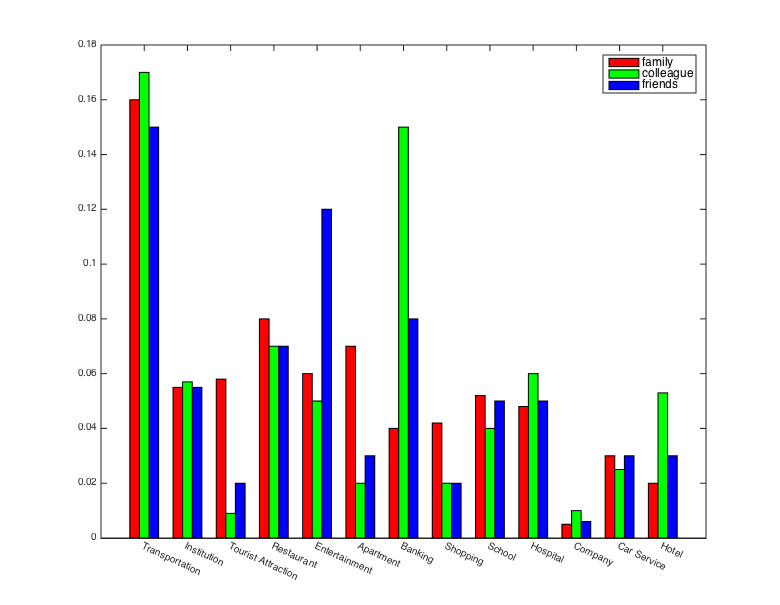
\includegraphics[scale=1, width=0.95\textwidth]{figure/contextDistribution.png}
    \caption{不同社交关系与位置同现语义之间的关系}
    \label{fig-spatial-context}
\end{figure}


在图\ref{fig-spatial-context}中本文可以观察到,具有家庭关系的用户出现在住宅区、旅游景点等地方。这也验证了本文更多愿意和家人出去旅游,或者在家里陪伴家人。另外,具有同事关系的用户出现在商业街或者酒店,这也反映出了同事们最常上班的地方即在商业街,或者一起出差去了酒店等等。这一粗略的分析也反映了具有不同社交关系的用户往往会选择在不同的地点进行聚集,这也粗略地反映了不同社交关系的群体往往具有不同的社交行为,和群交关系爱好。



\subsection{社交结构团分析}
在以前的很多研究中\upcite{tang2012inferring,dong2014inferring},都或多或少从社会学理论角度进行分析社交网络,社交平衡理论\upcite{easley2010networks}(Social Balance Theory)则是被成功运用到社交网络中的经典知识之一。社交平衡理论阐释在实际社交网络中,随着不同用户之间的交流增多,一个初始的网络最后往往会发展成稳定的网络,而且最终往往会形成比较稳定的网络结构。图\ref{fig-structral-balance}则为社交平衡理论在本文的移动社交网络中的实际应用。图中,本文采用三元团来举例社交平衡理论,也因为三元团是社交平衡理论中最简单的结构之一。对于一个三元团所构成的闭环,每一条边都代表社交网络中用户的关系,如在本文的网络中,每条边的关系可以是家庭、同事或者朋友。如此一来,在实际社交网络中所有可能存在此三元团结构为10中,正如图中所示。但是,社交平衡理论告诉本文,并不是所有的三元团都是稳定的,可保持的。随着时间的推移,网络拓扑图中不平衡的三元团会越来越少,而平衡的三元团会越来越多,理想情况下最终一个稳定的社交网络中只会存在极少数的不稳定三元团。



\begin{figure}[ht]
    \centering
    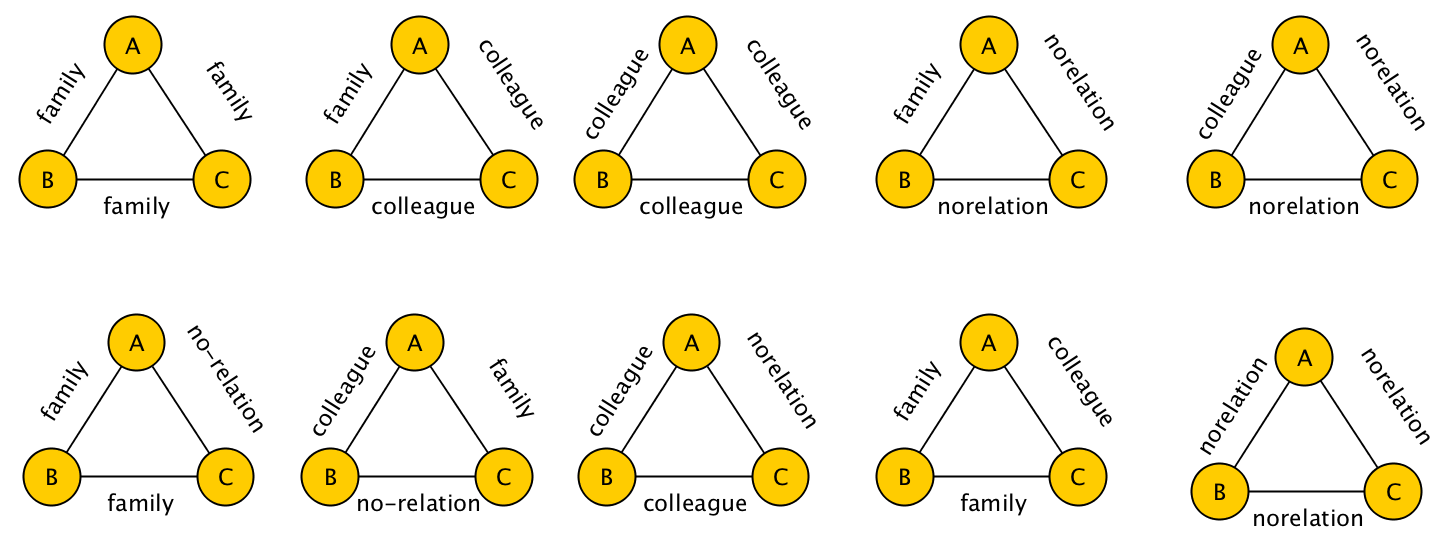
\includegraphics[scale=1, width=0.9\textwidth]{figure/relations.PNG}
    \caption{结构平衡理论举例}
    \label{fig-structral-balance}
\end{figure}


具体到本文的网络中实际分析,本文可以认为家庭关系、同事关系属于较强、比较稳定的关系类型,而朋友关系属于不稳定的关系类型(类似对比到一个仅仅由信任-不信任网络中,信任属于较强、较为稳定的关系类型,而不信任属于较弱、不稳定的关系类型)。但同时考虑家庭关系、同事关系的不同点,本文认为家庭关系比同事关系的稳定性更强(同事关系最终可能发展为家庭关系,也可能因为离职等因素而破坏)。以此类推,本文认为在所有的三元团里面,由三条边都是家庭关系、三条边都是同事关系、一条边是家庭关系和两条边是同事关系、一条边是家庭关系和两条边是朋友关系、一条边是同事关系和两条边是朋友关系所构成的三元结构团为稳定的三元团,而其他的都是不稳定的三元团。在此基础上,本文统计了哪些满足稳定条件的三元团在整个移动社交网络中所占的比例,看是否符合本文所提出的平衡理论。图清晰的展示了本文统计的结果。如图\ref{fig-structral-balance-stat},本文知道本文所认为具有平衡结构的三元团大约占了总的三元团85\%的比例,这也证明了在一个较为稳定的社交网络中,人们会逐渐形成较为稳定的结构,最终整个网络中所占的不稳定三元团总数相对来说较少。





\begin{figure}[ht]
    \centering
    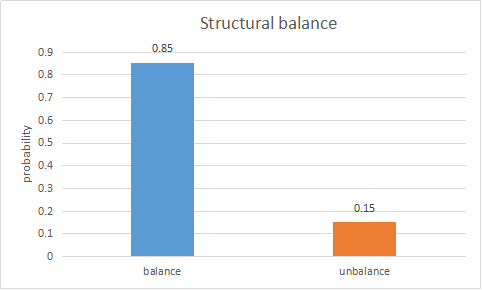
\includegraphics[scale=1, width=0.8\textwidth]{figure/structural_balance.PNG}
    \caption{平衡与不平衡三元团结构在社交网络中所占的比例}
    \label{fig-structral-balance-stat}
\end{figure}


由此延伸,本文将社交理论中的三元团进行扩展,放到真实世界中。本文分析这些在社交层面上具有的三元团,将三元团中的三个人同现的地理位置与时刻单独挑出来进行分析。由于篇幅的限制,本文这里不再展示结果,仅仅说一下思路。将具有三元团结构的用户提取出来,并分析他们同现的地方的地理语义,去其最常去的地方的地理语义,即为特征。这部分社交三元团、地理语义三元团与后面模型中的团特征相关。







